




\chapter{Base version}
\section{Problématiques}
\subsection{Le jeu}
 \label{sec1:le jeu}
 \textbf{Kitty Wonderland} est un jeu de cartes où au moins 2 joueurs s'affrontent sur un plateau de jeu. Chaque joueur a des points d'énergie (que l'on peut voir comme les points de vie) et une jauge d'idées (que l'on pourrait aussi désigné comme des points de mana) qui s'incrémentent d'un gain propre au joueur à chaque tour.\\
 Chaque joueur dispose d'une main de 5 cartes, avec un coût en matière d'idées pour chaque carte et une probabilité d'être tirée qui lui est propre. Les cartes disponibles sont:\\
 
 \hspace{-0,5cm} 
 \begin{tabularx}{15,2cm}{|c|c|X|c|}
 \hline 
 Carte & Coût & \multicolumn{1}{c}{Effet} & Probabilité  \\
 \hline
 Kitty Think & 5 & Augmente le gain du joueur de 1 & $\frac{20}{131}$ \rule[-7pt]{0pt}{20pt}  \\
 \hline 
 Kitty Steal & 10 & Augmente le gain du joueur de 1 et diminue celui de l'advervaire de 1  & $\frac{10}{131}$ \rule[-7pt]{0pt}{20pt}  \\
 \hline
 Kitty Panacea & 2 & Augmente l'énergie du joueur de 10 & $\frac{50}{131}$ \rule[-7pt]{0pt}{20pt}  \\
 \hline 
 Kitty Razor & 2 & Diminue l'énergie de l'adversaire de 10 & $\frac{50}{131}$ \rule[-7pt]{0pt}{20pt} \\
 \hline
 Kitty Hell is others & 100 & Diminue l'énergie de l'adversaire de INT\_MAX \footnote{INT\_MAX est l'entier maximal atteignable}& $\frac{1}{131}$ \rule[-7pt]{0pt}{20pt}\\
 \hline
 \end{tabularx}
 \vspace{0,2cm} \\
 \underline{Début de partie}:\\
 Au début du jeu, chaque joueur dispose de:\\
 50 points d'énergie, 0 idées, un gain de 1 et 5 cartes qui sont tirées aléatoirement dans le momento (Deck).\\
 \underline{Tour de jeu}:\\
 A chaque tour du jeu, chaque joueur met à jour sa jauge d'idées en fonction de son gain et choisit une carte selon ses idées: s'il en a suffisamment, il joue sa carte, déduit son coût de sa jauge d'idées et la défausse, sinon il passe son tour.
 À la fin du tour, chaque joueur reconstitue sa main en repiochant des cartes jusqu'à avoir de nouveau une main complète, et si un joueur a perdu tout ses points d'énergie, on le déclare perdant et il ne participe plus à la bataille.\\
 \\
 \underline{fin de la partie}:\\
 Le jeu prends fin lorsqu'il n'y a plus qu'un seul joueur, déclaré alors vainqueur ; ou lorsque tout le monde a été éliminés : partie nulle.
 
 
 
 
 
 
 
\subsection{Les impératifs}
La modélisation de ce jeu requiert différents points. Tout d'abord, il faut trouver une représentation propice des différents éléments: comment choisir les structures des joueurs, des cartes et du plateau de jeu? Quel type choisir pour modéliser la main du joueur? Ensuite, il faut conceptualiser les algorithmes gérant la dynamique du jeu pour qu'ils collent au fonctionnement attendu. De plus, il faut répartir ces fonctions dans plusieurs fichiers sources, et donc trouver un découpage adéquat. Ce découpage ne doit pas interférer avec les appels mutuels des fonctions à la compilation. Enfin, pour gérer la compilation séparée de ces fichiers et ne pas recompiler inutilement des fichiers non modifiés, il faut établir un Makefile gérant les compilations.











\section{Choix d'implémentation}
\subsection{Modélisation}
\label{sec1: modelisation}
La modélisation de ce jeu est basé sur des structures. \\
Une  carte est modélisée par une structure \textbf{card} qui contient les champs suivants :
\begin{itemize}
    \item  \textbf{id} : son identifiant
    \item \textbf{name} : son nom 
    \item \textbf{cost} : son coût 
    \item \textbf{gain-player} : le gain qu'elle offre au joueur 
    \item \textbf{gain-adversary} : le gain qu'elle prend à l'adversaire donc négative 
    \item \textbf{energy-player} : l'énergie qu'elle offre au joueur 
    \item \textbf{energy-adversary} : l'énergie qu'elle prend à l'adversaire :donc négative
 \end{itemize}
 
L'ensemble des cartes est catalogué dans le tableau \texttt{card\_list} contenant chacune des différentes cartes. Pour modéliser l'absence de cartes, on crée la carte fantôme supplémentaire "Null". Chaque carte à un identifiant, qui correspond à sa case dans \texttt{card\_list}. Ceci permet de confondre les cartes avec leur idendifiants, et ainsi travailler avec des entiers et non avec des structures lourdes.\\
\underline{Remarque} : une amélioration possible aurait été de travailler avec des pointeurs plutôt que des identifiants.\\
 \begin{tabularx}{16cm}{|c|c|c|X|X|X|X|X|}
 \hline 
 Carte & id & Coût & Gain Joueur & Gain\hspace{1cm}Adversaire & Énergie\hspace{1cm}Joueur & Énergie\hspace{1cm}Adversaire \\
 \hline
 Null & 0 & 0 & \multicolumn{1}{c|}{0} & \multicolumn{1}{c|}{0} & \multicolumn{1}{c|}{0} & \multicolumn{1}{c|}{0}  \\
 \hline 
 Kitty Think & 1 & 5 & \multicolumn{1}{c|}{1} & \multicolumn{1}{c|}{0} & \multicolumn{1}{c|}{0} & \multicolumn{1}{c|}{0}  \\
 \hline 
 Kitty Steal & 2 & 10 & \multicolumn{1}{c|}{1} & \multicolumn{1}{c|}{1} & \multicolumn{1}{c|}{0} & \multicolumn{1}{c|}{0} \\
 \hline
 Kitty Panacea & 3 & 2 & \multicolumn{1}{c|}{0} & \multicolumn{1}{c|}{0} & \multicolumn{1}{c|}{10} & \multicolumn{1}{c|}{0}\\
 \hline 
 Kitty Razor & 4 & 2 & \multicolumn{1}{c|}{0} & \multicolumn{1}{c|}{0} & \multicolumn{1}{c|}{0} & \multicolumn{1}{c|}{10} \\
 \hline
 Kitty Hell is others & 5 & 100 & \multicolumn{1}{c|}{0} & \multicolumn{1}{c|}{0} & \multicolumn{1}{c|}{0} & \multicolumn{1}{c|}{INT\_MAX} \\
 \hline
 \end{tabularx}
 
\vspace{1cm}

Le joueur est de même modélisé par une structure \textbf{player} qui contient les champs suivants :
\begin{itemize}
\item  \textbf{energy} son énergie
\item  \textbf{ideas} ses idées
\item  \textbf{gain} son gain
\item  \textbf{state} son état : mort ou vivant.
\item \textbf{hand} sa main sous forme d'un tableau qui contient les id de ses cartes 
\item \textbf{deck} son momento : c'est un pointeur. Ce champ a été ajouté lors de la réalisation de l'Achievement 1 pour avoir une compatibilité entre les deux versions (cf \ref{sec2:ach1}).
\end{itemize}

\vspace{1cm}

Enfin le plateau de jeu est modélisé par une structure qui contient les champs :
\begin{itemize}
    \item \textbf{number\_players} : le nombre des joueurs d'une partie.
    \item \textbf{players\_alive} : le nombre des joueurs vivants.
    \item \textbf{players} : tableau des joueurs. 
    \item \textbf{round} : le tour de jeu en cours.
\end{itemize}
Le champ round est incrémenté à chaque tour, et permet ainsi de stopper le jeu si la partie est trop longue.









\subsection{Le découpage des fichiers}
L'organisation du code se fait en plusieurs fichiers.\\
Le projet contient deux headers: \texttt{definition.h} qui contient les définitions des structures de base, et \texttt{fonctions.h} qui contient les prototypes des toutes les fonctions, permettant les appels mutuels des fonctions. Ces fonctions sont réparties dans trois fichiers source: \texttt{board.c}, \texttt{cards.c} et \texttt{deck.c} (ce dernier a été créé par la pour la compatibilité avec l'Achievement 1, cf \ref{sec2:ach1}). Enfin, tous ces éléments sont integrées avec les headers dans le fichiers \texttt{game.c} qui gère la boucle de jeu. Ils peuvent aussi être compilés avec les trois fichiers test, \texttt{test\_deck.c}, \texttt{test\_board.c}, et \texttt{test\_cards.c}, pour tester les fonctions prises individuellement (cf \ref{sec3: ftest}) .
\\*



\begin{figure}[h]
    \centering
    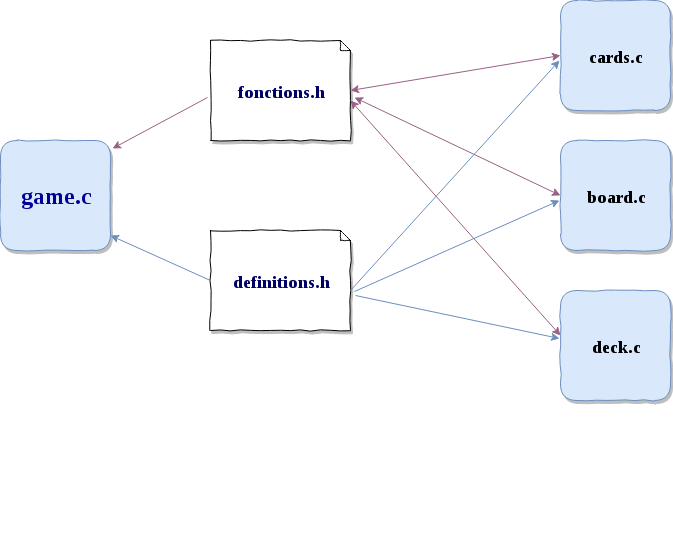
\includegraphics[width=1\textwidth]{./figures/organisation_bv.png}
    \caption{découpage des fichiers du Base version}
    \label{fig:Base_version_files}
\end{figure}




\subsection{Les fonctions du plateau de jeu}
\label{sec1: fboard}

\subsubsection{Fonctions d'initialisation du board:}
L'initialisation du plateau de jeu se fait à travers la fonction \texttt{init\_board} , on passe en paramètre le nombre de joueurs number\_players qui est aussi égal au début du jeu au nombre de joueurs en vie: players\_alive. Pour chacun des es joueurs, on initialise son états: state à 1, pour dire qu'il vivant en début de partie, son énergie à 50 points, son idées à 0, son gain à 1 et sa main vide. Enfin, on fait un tirage aléatoire de 5 cartes pour remplir sa main en faisant appel à la fonction \texttt{refill\_card} (cf \ref{sec1:fcards}) \\
\textbf{Complexité :}\\
Si on note n le nombre de joueurs passé en paramètre, alors puisque au sein de la fonction \texttt{init\_board} on fait un parcours complet du tableau des joueurs et on fait appel à la fonction \texttt{refill\_cards}, qui a une complexité constante (cf\ref{sec1:fcards}). Quant aux fonctions \texttt{init\_deck} et \texttt{distribute} qui sont aussi appelées par \texttt{init\_board}, elles ne font rien dans Base version ( cf(\ref{sec2:ach1})). Donc la fonction \texttt{init\_board} est de complexité linéaire par rapport au nombre de joueurs $\theta(n)$. 


\subsubsection{Fonctions de la dynamique du jeu:}
A chaque début de tour, il est nécessaire d'augmenter les idées de chaque joueur en fonction de son gain. D'où le besoin de la fonction: \texttt{Increase\_ideas}.
A la fin de chaque tour, il faut également vérifier si l'un des joueurs est mort \textit{i.e.} si son énergie est négative ou nulle, et si c'est le cas, le noté comme mort (changer son champ state pour 0) et décrémenter le nombre des joueurs en vie: c'est le rôle de la fonction \texttt{death}.\\
\textbf{Complexité :}\\
Les deux fonctions effectuent un parcours complet du tableau des joueurs pour modifier les champs des joueurs, auxquels elles ont accès en temps constant. Elles s'effectuent donc en $\theta(n)$.


\subsubsection{Affichage:}
 Les dernières fonctions se rapportant au plateau de jeu sont des fonctions d'affichage :\texttt{display\_players} et  \texttt{announce\_results}, permettant respectivement d'afficher l'état de la partie en fin de chaque tour, et d'annoncer le résultat à la fin de la partie. La parti se finit lorsqu'il y a moins de 2 joueurs ou lorsque le maximum de tours de jeu est atteint.\\
\textbf{Complexité :}\\
En cas de match nul ou de dépassement du nombre de tours autorisés, la fonction \texttt{announce\_results}  a accès aux données nécessaire à l'annonce du résultat en temps constant par le board. Sinon, elle dois parcourir le tableau des joueurs pour trouver le vainqueur et s'effectue donc en $\theta(n)$. Elle est donc en $\mathcal{O}(n)$.







\subsection{Les fonctions des cartes}
\label{sec1:fcards}

\subsubsection{Les choix aléatoires:}

Le jeu est grandement basé sur l'utilisation aléatoire des cartes : chaque carte est piochée et jouée de façon aléatoire (dans la mesure des règles d'utilisation). Il est donc nécessaire de créer une fonction \texttt{random\_card}. La génération aléatoire de chacune des cartes, en respectant les règles de probabilités énoncées plus haut (cf \ref{sec1:le jeu}).\\
Pour cela on génère un nombre r àléatoire entre 0 et 130 : \\
si r $\in$ [0,20[, alors c'est la carte Kitty Think \\
si r $\in$ [20,30[, alors c'est la carte Kitty Steal \\
si r $\in$ [30,80[, alors c'est la carte Kitty Razor \\
si r $\in$ [80,130[, alors c'est la carte Kitty Panaceas \\
si r = 130, alors c'est la carte Kitty Hell is Other \\ \\
Cette fonction permet le tirage aléatoire d'une carte parmi les 5 proposées. Cependant, pour des raisons de compatibilité entre l'Achievement 1 et la Base version (cf \ref{sec2:ach1}), elle n'est pas appelée directement pour le tirage d'une carte, mais elle est appelée dans la fonction wrap \texttt{draw\_card}, qui est la seule fonction non vide de \texttt{deck.c}.\\
\textbf{Complexité :}\\
La génération d'une carte aléatoire est en temps constant, $\theta(1)$.\\



Il est aussi nécessaire de choisir un adversaire de façon aléatoire. Le choix de cet adversaire ce fait dans \texttt{choose\_adversary} selon l'algorithme suivant : 



\begin{algorithm}
\caption{algorithme du choix de l'adversaire}
\begin{algorithmic} 
\REQUIRE joueur numéro p ; n joueurs, a joueurs vivants\\
\COMMENT{//le joueur peut choisir parmi les a-1 candidats, \textit{i.e.}les joueurs vivants autres que lui : il choisit le r\up{ème} joueur dans cet ensemble des façon aléatoire}\\
\STATE $r \leftarrow $ random[0,a-1]\\
\COMMENT {//on cherche le numéro adv correspondant au r\up{ème} candidats}\\
\COMMENT{//d'abord, on passe les r candidats précédants}\\
\WHILE{$ r \neq 0$ }
\IF{adv est un candidat}
\STATE $r\leftarrow r - 1$
\ENDIF
\STATE $adv \leftarrow adv + 1$
\ENDWHILE\\
\COMMENT{//à présent, le premier joueur vivant autre que p est le bon advesaire}\\
\WHILE{adv n'est pas un candidat}
\STATE $adv \leftarrow adv + 1$
\ENDWHILE
\end{algorithmic}
\end{algorithm}

\noindent \underline{Remarque}: \\
Dans l'algorithme, on a forcément a-1\textgreater0 car pour entrer dans la boucle de jeux, le nombre de joueur doit être $\geq 2$ (sinon la partie se serait achevée au tour d'avant), et la procédure de mort n'est appelée qu'à la fin du tour.\\
Prenons par exemple la situation de la figure \ref{fig:choose_adversary} : il y a 10 joueurs parmi lesquels les joueurs 1, 2 et 6 sont morts. Le joueur 8 peut donc choisir parmi les 6 joueurs 0, 3, 4, 5, 7 et 9. Ces derniers sont renumérotés de 0 à 5 pour le tirage aléatoire, le but de l'algorithme et de retrouver la correspondance entre le numéro tiré et l'identifiant du joueur.\\
\begin{figure}
    \centering
    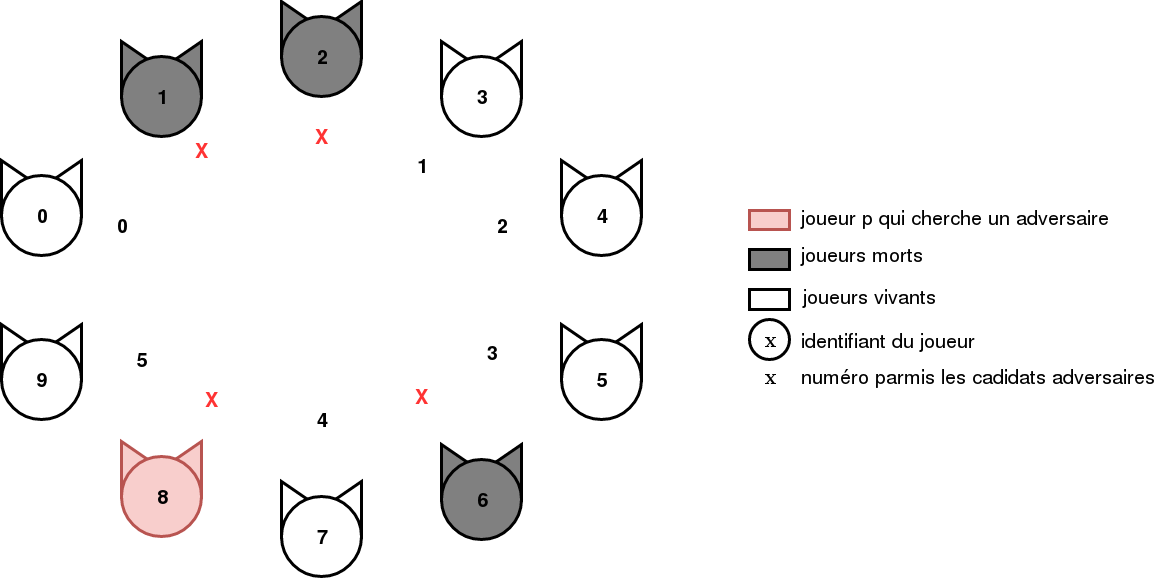
\includegraphics[width=1\textwidth]{./figures/choose_adversary.png}
    \caption{exemple de situation de choix d'un adversaire}
    \label{fig:choose_adversary}
\end{figure}
\noindent \textbf{Complexité:}\\
Dans le pire des cas, la fonction va devoir parcourir tout le tableau de joueurs pour trouver l'adversaire. Elle s'effectue donc en $\mathcal{O}(n)$.






\subsubsection{Les fonctions dynamiques des cartes:}

A chaque tour, chaque joueur choisit une carte: il choisit la première de sa main que lui permettent ses idées selon son coût. Ceci est réalisé dans \texttt{select\_card}. Le choix de la carte jouée est bien aléatoire puisque les cartes arrivent de façon aléatoire dans sa main avec \texttt{draw\_card}.\\
\textbf{Complexité :}\\
Le choix de la carte nécessite dans le pire des cas un parcours complet de la main en faisant appel à des instructions et des fonctions réalisées en temps constant, mais comme la main est de taille constante (5 cartes), la complexité de \texttt{select\_card} est en $\theta(1)$. \\


Une fois que la carte et l'adversaire sont choisis, il faut appliquer les effets de la carte au joueur et à son adversaire, c'est le rôle de \texttt{apply\_card}.\\
\texttt{Complexité :}\\
Elle agit sur les champs des joueurs qui sont des action en temps constant, mais c'est elle qui appelle \texttt{choose\_adversary} qui est en  $\theta(n)$ , donc elle l'est également.\\


Enfin, à la fin de chaque tour, le joueur rempli sa main grâce à \texttt{refill\_cards}. Cette dernière parcourt la main du joueur pour trouver les emplacements vides est appeler \textbf{draw\_card} si tel est le cas.\\
\textbf{Complexité:}\\
\texttt{draw\_card} est de complexité constante et la main est de taille fini donc le remplissage de la main se fait en temps constant.














